\documentclass{beamer}

\pdfmapfile{+sansmathaccent.map}


\mode<presentation>
{
  \usetheme{Warsaw} % or try Darmstadt, Madrid, Warsaw, Rochester, CambridgeUS, ...
  \usecolortheme{seahorse} % or try seahorse, beaver, crane, wolverine, ...
  \usefonttheme{serif}  % or try serif, structurebold, ...
  \setbeamertemplate{navigation symbols}{}
  \setbeamertemplate{caption}[numbered]
} 


%%%%%%%%%%%%%%%%%%%%%%%%%%%%
% itemize settings

\definecolor{mypink}{RGB}{255, 150, 150}
\definecolor{myblue}{RGB}{150, 150, 255}
\definecolor{mygray}{gray}{0.8}

\setbeamertemplate{itemize items}[default]

\setbeamertemplate{itemize item}{\color{mypink}$\blacksquare$}
\setbeamertemplate{itemize subitem}{\color{myblue}$\blacktriangleright$}
\setbeamertemplate{itemize subsubitem}{\color{mygray}$\blacksquare$}

%%%%%%%%%%%%%%%%%%%%%%%%%%%%
% block settings

\setbeamercolor{block title}{bg=red!30,fg=black}


%%%%%%%%%%%%%%%%%%%%%%%%%%%%
% URL settings
\hypersetup{
    colorlinks=true,
    linkcolor=blue,
    filecolor=blue,      
    urlcolor=blue,
}

%%%%%%%%%%%%%%%%%%%%%%%%%%

\renewcommand{\familydefault}{\rmdefault}

\usepackage{amsmath}
\usepackage{mathtools}

\DeclareMathOperator*{\argmin}{arg\,min}

\usepackage{subcaption}




%%%%%%%%%%%%%%%%%%%%%%%%%%%%
% code settings

\usepackage{listings}
\usepackage{color}
\definecolor{mygreen}{rgb}{0,0.6,0}
\definecolor{mygray}{rgb}{0.5,0.5,0.5}
\definecolor{mymauve}{rgb}{0.58,0,0.82}
\lstset{ 
  backgroundcolor=\color{white},   % choose the background color; you must add \usepackage{color} or \usepackage{xcolor}; should come as last argument
  basicstyle=\footnotesize,        % the size of the fonts that are used for the code
  breakatwhitespace=false,         % sets if automatic breaks should only happen at whitespace
  breaklines=true,                 % sets automatic line breaking
  captionpos=b,                    % sets the caption-position to bottom
  commentstyle=\color{mygreen},    % comment style
  deletekeywords={...},            % if you want to delete keywords from the given language
  escapeinside={\%*}{*)},          % if you want to add LaTeX within your code
  extendedchars=true,              % lets you use non-ASCII characters; for 8-bits encodings only, does not work with UTF-8
  firstnumber=0000,                % start line enumeration with line 0000
  frame=single,	                   % adds a frame around the code
  keepspaces=true,                 % keeps spaces in text, useful for keeping indentation of code (possibly needs columns=flexible)
  keywordstyle=\color{blue},       % keyword style
  language=Octave,                 % the language of the code
  morekeywords={*,...},            % if you want to add more keywords to the set
  numbers=left,                    % where to put the line-numbers; possible values are (none, left, right)
  numbersep=5pt,                   % how far the line-numbers are from the code
  numberstyle=\tiny\color{mygray}, % the style that is used for the line-numbers
  rulecolor=\color{black},         % if not set, the frame-color may be changed on line-breaks within not-black text (e.g. comments (green here))
  showspaces=false,                % show spaces everywhere adding particular underscores; it overrides 'showstringspaces'
  showstringspaces=false,          % underline spaces within strings only
  showtabs=false,                  % show tabs within strings adding particular underscores
  stepnumber=2,                    % the step between two line-numbers. If it's 1, each line will be numbered
  stringstyle=\color{mymauve},     % string literal style
  tabsize=2,	                   % sets default tabsize to 2 spaces
  title=\lstname                   % show the filename of files included with \lstinputlisting; also try caption instead of title
}

%%%%%%%%%%%%%%%%%%%%%%%%%%%%
% tikz settings

\usepackage{tikz}
\tikzset{every picture/.style={line width=0.75pt}}


\title{Introduction}
\subtitle{Contact-aware Control, Lecture 1}
\author{by Sergei Savin}
\centering
\date{Fall 2020}



\begin{document}
\maketitle


\begin{frame}{Content}

\begin{itemize}
\item Motivation
\item Contact in Robotics
\item Motivating example
\begin{itemize}
\item Two body oscillator, part 1-4
\end{itemize}
\item This course
\begin{itemize}
\item Content
\item Tools we will use and learn
\end{itemize}


\end{itemize}

\end{frame}



\begin{frame}{Motivation}
\framesubtitle{Dynamics depends on contact}
\begin{flushleft}

\begin{figure}
\minipage{0.32\textwidth}
  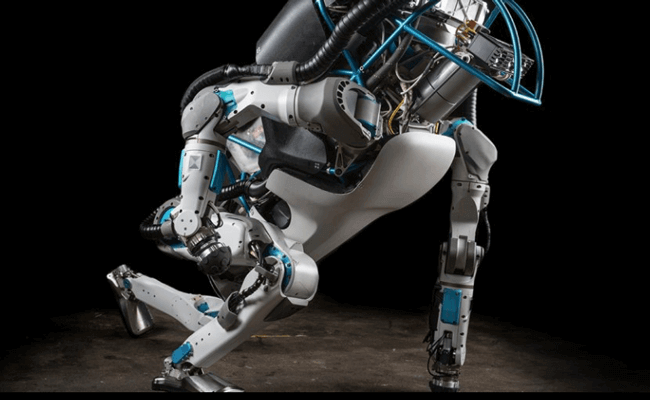
\includegraphics[width=\linewidth]{Atlas-Bot.png}
\endminipage\hfill
\minipage{0.42\textwidth}
  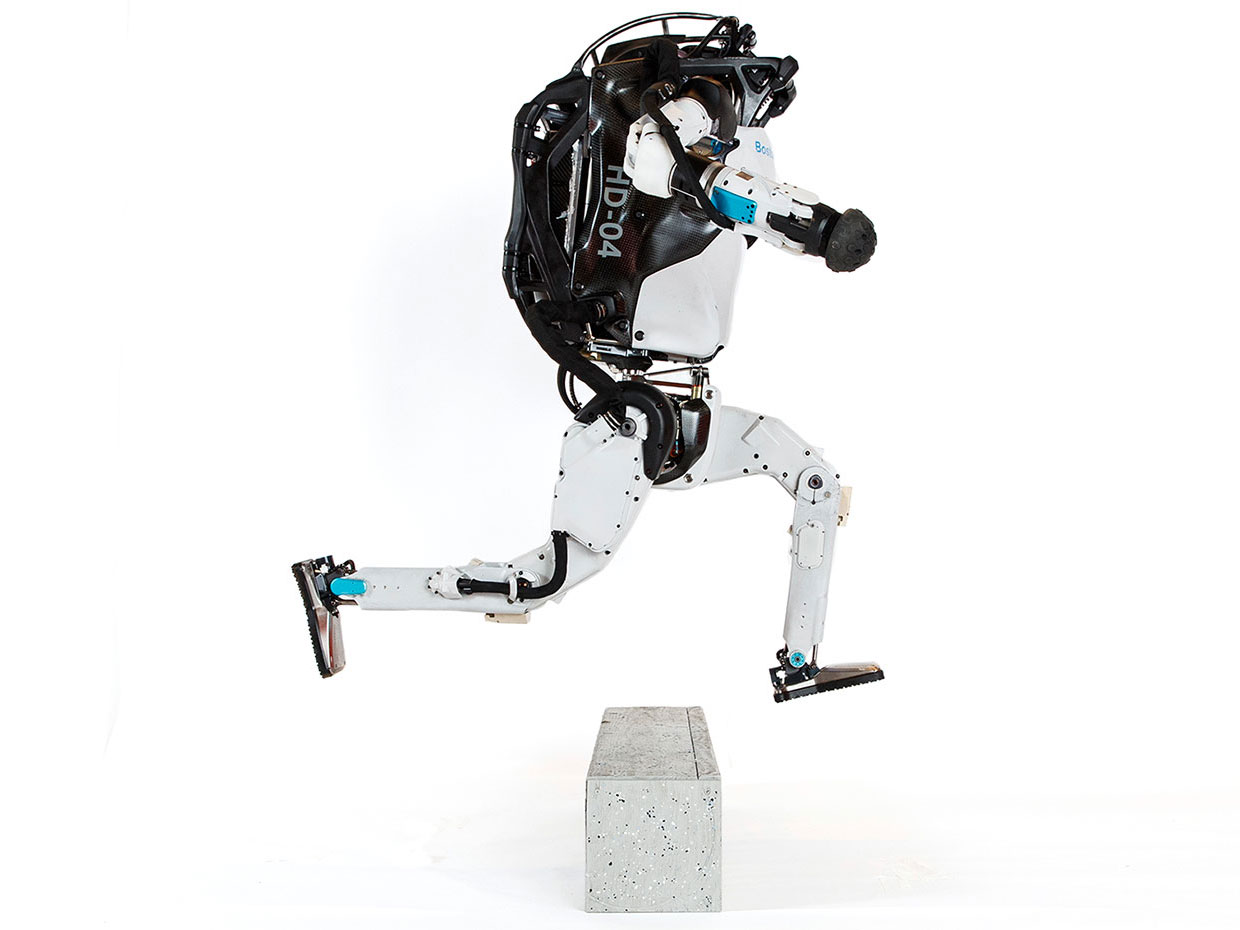
\includegraphics[width=\linewidth]{atlas in the air.jpeg}
\endminipage\hfill
\minipage{0.22\textwidth}%
  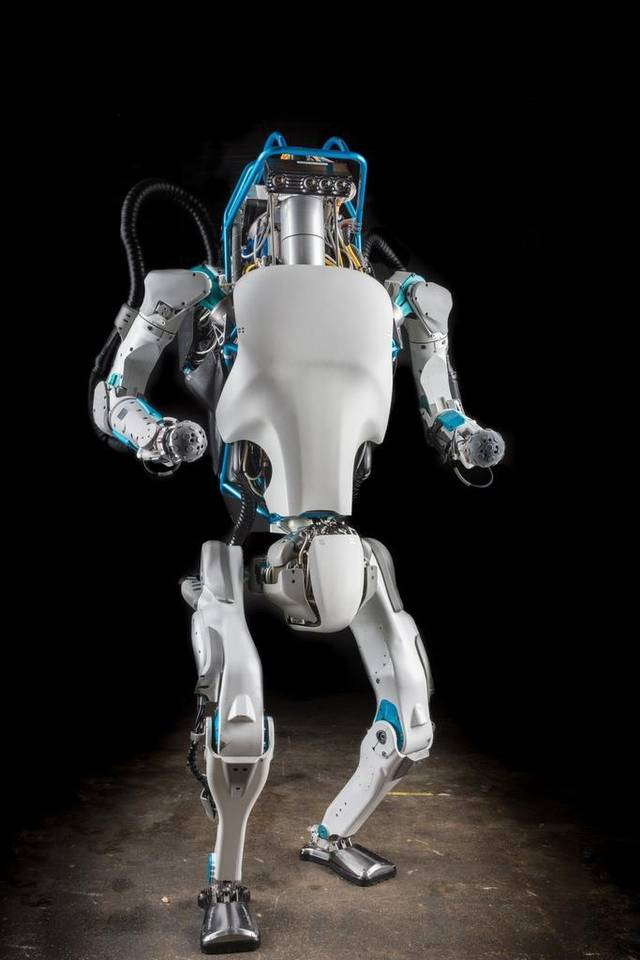
\includegraphics[width=\linewidth]{Atlas_from_boston_dynamics.jpg}
\endminipage

\end{figure}

\bigskip

What do you find different between those poses in terms of mobility of the robot? 

\end{flushleft}
\end{frame}


\begin{frame}{Contact in Robotics}
% \framesubtitle{Parameter estimation}
\begin{flushleft}

There are a number of areas where changes in contact interaction between the robot and the environment is part of normal operation of the robot:

\bigskip

\begin{itemize}
    \item walking robots;
    \item collaborative robots;
    \item robots performing tooling and other operations which do not involve moving the operated objects.
\end{itemize}

\end{flushleft}
\end{frame}



\begin{frame}{Motivating example}
\framesubtitle{Two body oscillator, part 1}
\begin{flushleft}

\begin{figure}
    \centering
    
\tikzset{every picture/.style={line width=0.75pt}} %set default line width to 0.75pt        

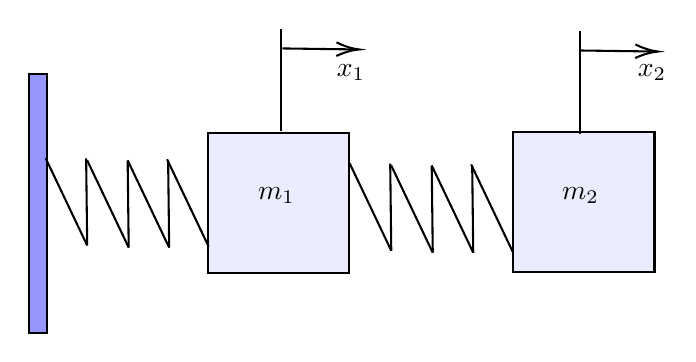
\begin{tikzpicture}[x=0.75pt,y=0.75pt,yscale=-1,xscale=1]
%uncomment if require: \path (0,300); %set diagram left start at 0, and has height of 300

%Shape: Rectangle [id:dp6193525951241812] 
\draw  [fill=myblue  ,fill opacity=0.18 ] (114.5,70.5) -- (182.5,70.5) -- (182.5,137.83) -- (114.5,137.83) -- cycle ;
%Shape: Rectangle [id:dp2754614534814892] 
\draw  [fill=myblue  ,fill opacity=1 ] (28,42) -- (36.67,42) -- (36.67,166.5) -- (28,166.5) -- cycle ;
%Straight Lines [id:da24513887248814736] 
\draw    (36.17,82.5) -- (56.17,124.5) ;
%Straight Lines [id:da6389992822273287] 
\draw    (56.17,124.5) -- (55.67,82.58) ;
%Straight Lines [id:da6096744543318782] 
\draw    (56.17,83.5) -- (76.17,125.5) ;
%Straight Lines [id:da01129832742067105] 
\draw    (76.17,125.5) -- (75.67,83.58) ;
%Straight Lines [id:da22449274713248912] 
\draw    (75.67,83.5) -- (95.67,125.5) ;
%Straight Lines [id:da8276213296972594] 
\draw    (95.67,125.5) -- (95.17,83.58) ;
%Straight Lines [id:da498962233361786] 
\draw    (94.67,83) -- (114.67,125) ;
%Straight Lines [id:da46232618249152724] 
\draw    (182.67,85) -- (202.67,127) ;
%Straight Lines [id:da7579720932367997] 
\draw    (202.67,127) -- (202.17,85.08) ;
%Straight Lines [id:da40612218699006064] 
\draw    (202.67,86) -- (222.67,128) ;
%Straight Lines [id:da11178597500061249] 
\draw    (222.67,128) -- (222.17,86.08) ;
%Straight Lines [id:da7928381793295927] 
\draw    (222.17,86) -- (242.17,128) ;
%Straight Lines [id:da4171044513027511] 
\draw    (242.17,128) -- (241.67,86.08) ;
%Straight Lines [id:da20128280842481572] 
\draw    (241.17,85.5) -- (261.17,127.5) ;
%Straight Lines [id:da11261786423812614] 
\draw    (149.67,69.58) -- (149.67,20.08) ;
%Straight Lines [id:da16787925759193145] 
\draw    (150.17,29.58) -- (185.17,30.06) ;
\draw [shift={(187.17,30.08)}, rotate = 180.77] [color={rgb, 255:red, 0; green, 0; blue, 0 }  ][line width=0.75]    (10.93,-3.29) .. controls (6.95,-1.4) and (3.31,-0.3) .. (0,0) .. controls (3.31,0.3) and (6.95,1.4) .. (10.93,3.29)   ;
%Straight Lines [id:da5475157311152137] 
\draw    (293.67,70.58) -- (293.67,21.08) ;
%Straight Lines [id:da23835845671995415] 
\draw    (294.17,30.58) -- (329.17,31.06) ;
\draw [shift={(331.17,31.08)}, rotate = 180.77] [color={rgb, 255:red, 0; green, 0; blue, 0 }  ][line width=0.75]    (10.93,-3.29) .. controls (6.95,-1.4) and (3.31,-0.3) .. (0,0) .. controls (3.31,0.3) and (6.95,1.4) .. (10.93,3.29)   ;
%Shape: Rectangle [id:dp6303797162561124] 
\draw  [fill=myblue  ,fill opacity=0.18 ] (261.5,70) -- (329.5,70) -- (329.5,137.33) -- (261.5,137.33) -- cycle ;

% Text Node
\draw (175, 36) node [anchor=north west][inner sep=0.75pt]    {$x_{1}$};
% Text Node
\draw (320, 36) node [anchor=north west][inner sep=0.75pt]    {$x_{2}$};
% Text Node
\draw (137, 95) node [anchor=north west][inner sep=0.75pt]    {$m_{1}$};
% Text Node
\draw (283.5, 95) node [anchor=north west][inner sep=0.75pt]    {$m_{2}$};

\end{tikzpicture}


    \caption{Two body oscillator diagram}
    \label{fig:my_label}
\end{figure}

This is an example of a system that you know how to describe:

\begin{equation}
\begin{cases}
    m_1 \ddot x_1 = k_1 x_1 + k_2 (x_2 - x_1 - l_{12}) \\
    m_2 \ddot x_2 = -k_2 (x_2 - x_1 - l_{12})
\end{cases}
\end{equation}

\end{flushleft}
\end{frame}



\begin{frame}{Motivating example}
\framesubtitle{Two body oscillator, part 2}
\begin{flushleft}

\begin{figure}
    \centering
    


\tikzset{every picture/.style={line width=0.75pt}} %set default line width to 0.75pt        

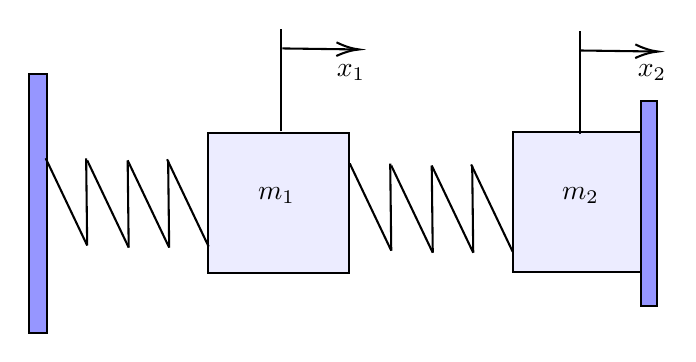
\begin{tikzpicture}[x=0.75pt,y=0.75pt,yscale=-1,xscale=1]
%uncomment if require: \path (0,300); %set diagram left start at 0, and has height of 300

%Shape: Rectangle [id:dp6193525951241812] 
\draw  [fill=myblue  ,fill opacity=0.18 ] (114.5,70.5) -- (182.5,70.5) -- (182.5,137.83) -- (114.5,137.83) -- cycle ;
%Shape: Rectangle [id:dp2754614534814892] 
\draw  [fill=myblue  ,fill opacity=1 ] (28,42) -- (36.67,42) -- (36.67,166.5) -- (28,166.5) -- cycle ;
%Straight Lines [id:da24513887248814736] 
\draw    (36.17,82.5) -- (56.17,124.5) ;
%Straight Lines [id:da6389992822273287] 
\draw    (56.17,124.5) -- (55.67,82.58) ;
%Straight Lines [id:da6096744543318782] 
\draw    (56.17,83.5) -- (76.17,125.5) ;
%Straight Lines [id:da01129832742067105] 
\draw    (76.17,125.5) -- (75.67,83.58) ;
%Straight Lines [id:da22449274713248912] 
\draw    (75.67,83.5) -- (95.67,125.5) ;
%Straight Lines [id:da8276213296972594] 
\draw    (95.67,125.5) -- (95.17,83.58) ;
%Straight Lines [id:da498962233361786] 
\draw    (94.67,83) -- (114.67,125) ;
%Straight Lines [id:da46232618249152724] 
\draw    (182.67,85) -- (202.67,127) ;
%Straight Lines [id:da7579720932367997] 
\draw    (202.67,127) -- (202.17,85.08) ;
%Straight Lines [id:da40612218699006064] 
\draw    (202.67,86) -- (222.67,128) ;
%Straight Lines [id:da11178597500061249] 
\draw    (222.67,128) -- (222.17,86.08) ;
%Straight Lines [id:da7928381793295927] 
\draw    (222.17,86) -- (242.17,128) ;
%Straight Lines [id:da4171044513027511] 
\draw    (242.17,128) -- (241.67,86.08) ;
%Straight Lines [id:da20128280842481572] 
\draw    (241.17,85.5) -- (261.17,127.5) ;
%Straight Lines [id:da11261786423812614] 
\draw    (149.67,69.58) -- (149.67,20.08) ;
%Straight Lines [id:da16787925759193145] 
\draw    (150.17,29.58) -- (185.17,30.06) ;
\draw [shift={(187.17,30.08)}, rotate = 180.77] [color={rgb, 255:red, 0; green, 0; blue, 0 }  ][line width=0.75]    (10.93,-3.29) .. controls (6.95,-1.4) and (3.31,-0.3) .. (0,0) .. controls (3.31,0.3) and (6.95,1.4) .. (10.93,3.29)   ;
%Straight Lines [id:da5475157311152137] 
\draw    (293.67,70.58) -- (293.67,21.08) ;
%Straight Lines [id:da23835845671995415] 
\draw    (294.17,30.58) -- (329.17,31.06) ;
\draw [shift={(331.17,31.08)}, rotate = 180.77] [color={rgb, 255:red, 0; green, 0; blue, 0 }  ][line width=0.75]    (10.93,-3.29) .. controls (6.95,-1.4) and (3.31,-0.3) .. (0,0) .. controls (3.31,0.3) and (6.95,1.4) .. (10.93,3.29)   ;
%Shape: Rectangle [id:dp6303797162561124] 
\draw  [fill=myblue  ,fill opacity=0.18 ] (261.5,70) -- (329.5,70) -- (329.5,137.33) -- (261.5,137.33) -- cycle ;
%Shape: Rectangle [id:dp9677043492583735] 
\draw  [fill=myblue  ,fill opacity=1 ] (323,55) -- (330.67,55) -- (330.67,153.5) -- (323,153.5) -- cycle ;

% Text Node
\draw (175, 36) node [anchor=north west][inner sep=0.75pt]    {$x_{1}$};
% Text Node
\draw (320, 36) node [anchor=north west][inner sep=0.75pt]    {$x_{2}$};
% Text Node
\draw (137, 95) node [anchor=north west][inner sep=0.75pt]    {$m_{1}$};
% Text Node
\draw (283.5, 95) node [anchor=north west][inner sep=0.75pt]    {$m_{2}$};


\end{tikzpicture}
    \caption{Two body oscillator diagram}
\end{figure}

Now we add a constraint:

\begin{equation}
x_2 = \text{const}
\end{equation}

How do we describe this one?

\end{flushleft}
\end{frame}



\begin{frame}{Motivating example}
\framesubtitle{Two body oscillator, part 3}
\begin{flushleft}

\begin{figure}
    \centering
    


\tikzset{every picture/.style={line width=0.75pt}} %set default line width to 0.75pt        

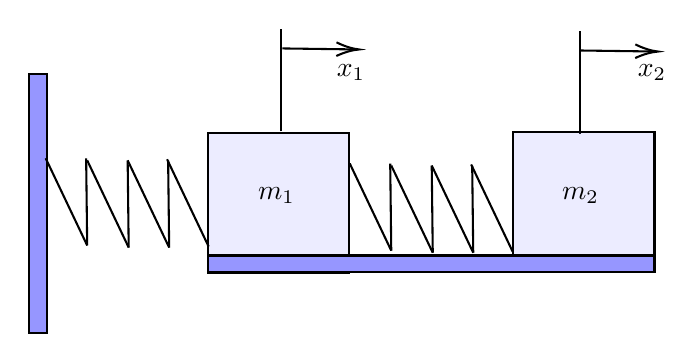
\begin{tikzpicture}[x=0.75pt,y=0.75pt,yscale=-1,xscale=1]
%uncomment if require: \path (0,300); %set diagram left start at 0, and has height of 300

%Shape: Rectangle [id:dp6193525951241812] 
\draw  [fill=myblue  ,fill opacity=0.18 ] (114.5,70.5) -- (182.5,70.5) -- (182.5,137.83) -- (114.5,137.83) -- cycle ;
%Shape: Rectangle [id:dp2754614534814892] 
\draw  [fill=myblue  ,fill opacity=1 ] (28,42) -- (36.67,42) -- (36.67,166.5) -- (28,166.5) -- cycle ;
%Straight Lines [id:da24513887248814736] 
\draw    (36.17,82.5) -- (56.17,124.5) ;
%Straight Lines [id:da6389992822273287] 
\draw    (56.17,124.5) -- (55.67,82.58) ;
%Straight Lines [id:da6096744543318782] 
\draw    (56.17,83.5) -- (76.17,125.5) ;
%Straight Lines [id:da01129832742067105] 
\draw    (76.17,125.5) -- (75.67,83.58) ;
%Straight Lines [id:da22449274713248912] 
\draw    (75.67,83.5) -- (95.67,125.5) ;
%Straight Lines [id:da8276213296972594] 
\draw    (95.67,125.5) -- (95.17,83.58) ;
%Straight Lines [id:da498962233361786] 
\draw    (94.67,83) -- (114.67,125) ;
%Straight Lines [id:da46232618249152724] 
\draw    (182.67,85) -- (202.67,127) ;
%Straight Lines [id:da7579720932367997] 
\draw    (202.67,127) -- (202.17,85.08) ;
%Straight Lines [id:da40612218699006064] 
\draw    (202.67,86) -- (222.67,128) ;
%Straight Lines [id:da11178597500061249] 
\draw    (222.67,128) -- (222.17,86.08) ;
%Straight Lines [id:da7928381793295927] 
\draw    (222.17,86) -- (242.17,128) ;
%Straight Lines [id:da4171044513027511] 
\draw    (242.17,128) -- (241.67,86.08) ;
%Straight Lines [id:da20128280842481572] 
\draw    (241.17,85.5) -- (261.17,127.5) ;
%Straight Lines [id:da11261786423812614] 
\draw    (149.67,69.58) -- (149.67,20.08) ;
%Straight Lines [id:da16787925759193145] 
\draw    (150.17,29.58) -- (185.17,30.06) ;
\draw [shift={(187.17,30.08)}, rotate = 180.77] [color={rgb, 255:red, 0; green, 0; blue, 0 }  ][line width=0.75]    (10.93,-3.29) .. controls (6.95,-1.4) and (3.31,-0.3) .. (0,0) .. controls (3.31,0.3) and (6.95,1.4) .. (10.93,3.29)   ;
%Straight Lines [id:da5475157311152137] 
\draw    (293.67,70.58) -- (293.67,21.08) ;
%Straight Lines [id:da23835845671995415] 
\draw    (294.17,30.58) -- (329.17,31.06) ;
\draw [shift={(331.17,31.08)}, rotate = 180.77] [color={rgb, 255:red, 0; green, 0; blue, 0 }  ][line width=0.75]    (10.93,-3.29) .. controls (6.95,-1.4) and (3.31,-0.3) .. (0,0) .. controls (3.31,0.3) and (6.95,1.4) .. (10.93,3.29)   ;
%Shape: Rectangle [id:dp6303797162561124] 
\draw  [fill=myblue  ,fill opacity=0.18 ] (261.5,70) -- (329.5,70) -- (329.5,137.33) -- (261.5,137.33) -- cycle ;
%Shape: Rectangle [id:dp9677043492583735] 
\draw  [fill=myblue  ,fill opacity=1 ] (114.5,129.33) -- (329.5,129.33) -- (329.5,137.33) -- (114.5,137.33) -- cycle ;


% Text Node
\draw (175, 36) node [anchor=north west][inner sep=0.75pt]    {$x_{1}$};
% Text Node
\draw (320, 36) node [anchor=north west][inner sep=0.75pt]    {$x_{2}$};
% Text Node
\draw (137, 95) node [anchor=north west][inner sep=0.75pt]    {$m_{1}$};
% Text Node
\draw (283.5, 95) node [anchor=north west][inner sep=0.75pt]    {$m_{2}$};


\end{tikzpicture}

    \caption{Two body oscillator diagram}
\end{figure}

Now we add a different constraint:

\begin{equation}
x_2 - x_1 = \text{const}
\end{equation}

How do we describe this one?

\end{flushleft}
\end{frame}




\begin{frame}{Motivating example}
\framesubtitle{Two body oscillator, part 4}
\begin{flushleft}

\begin{figure}
    \centering
    


\tikzset{every picture/.style={line width=0.75pt}} %set default line width to 0.75pt        

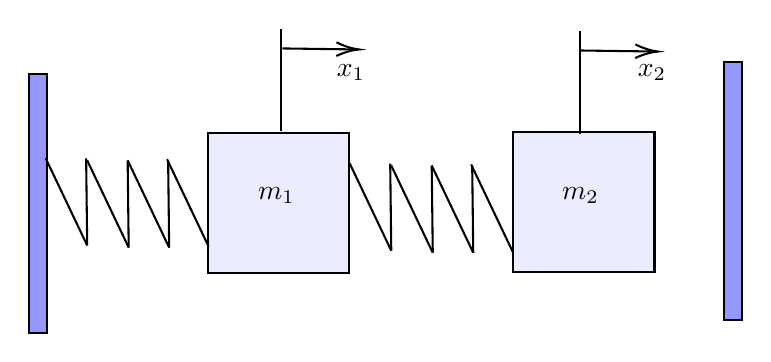
\begin{tikzpicture}[x=0.75pt,y=0.75pt,yscale=-1,xscale=1]
%uncomment if require: \path (0,300); %set diagram left start at 0, and has height of 300

%Shape: Rectangle [id:dp6193525951241812] 
\draw  [fill=myblue  ,fill opacity=0.18 ] (114.5,70.5) -- (182.5,70.5) -- (182.5,137.83) -- (114.5,137.83) -- cycle ;
%Shape: Rectangle [id:dp2754614534814892] 
\draw  [fill=myblue  ,fill opacity=1 ] (28,42) -- (36.67,42) -- (36.67,166.5) -- (28,166.5) -- cycle ;
%Straight Lines [id:da24513887248814736] 
\draw    (36.17,82.5) -- (56.17,124.5) ;
%Straight Lines [id:da6389992822273287] 
\draw    (56.17,124.5) -- (55.67,82.58) ;
%Straight Lines [id:da6096744543318782] 
\draw    (56.17,83.5) -- (76.17,125.5) ;
%Straight Lines [id:da01129832742067105] 
\draw    (76.17,125.5) -- (75.67,83.58) ;
%Straight Lines [id:da22449274713248912] 
\draw    (75.67,83.5) -- (95.67,125.5) ;
%Straight Lines [id:da8276213296972594] 
\draw    (95.67,125.5) -- (95.17,83.58) ;
%Straight Lines [id:da498962233361786] 
\draw    (94.67,83) -- (114.67,125) ;
%Straight Lines [id:da46232618249152724] 
\draw    (182.67,85) -- (202.67,127) ;
%Straight Lines [id:da7579720932367997] 
\draw    (202.67,127) -- (202.17,85.08) ;
%Straight Lines [id:da40612218699006064] 
\draw    (202.67,86) -- (222.67,128) ;
%Straight Lines [id:da11178597500061249] 
\draw    (222.67,128) -- (222.17,86.08) ;
%Straight Lines [id:da7928381793295927] 
\draw    (222.17,86) -- (242.17,128) ;
%Straight Lines [id:da4171044513027511] 
\draw    (242.17,128) -- (241.67,86.08) ;
%Straight Lines [id:da20128280842481572] 
\draw    (241.17,85.5) -- (261.17,127.5) ;
%Straight Lines [id:da11261786423812614] 
\draw    (149.67,69.58) -- (149.67,20.08) ;
%Straight Lines [id:da16787925759193145] 
\draw    (150.17,29.58) -- (185.17,30.06) ;
\draw [shift={(187.17,30.08)}, rotate = 180.77] [color={rgb, 255:red, 0; green, 0; blue, 0 }  ][line width=0.75]    (10.93,-3.29) .. controls (6.95,-1.4) and (3.31,-0.3) .. (0,0) .. controls (3.31,0.3) and (6.95,1.4) .. (10.93,3.29)   ;
%Straight Lines [id:da5475157311152137] 
\draw    (293.67,70.58) -- (293.67,21.08) ;
%Straight Lines [id:da23835845671995415] 
\draw    (294.17,30.58) -- (329.17,31.06) ;
\draw [shift={(331.17,31.08)}, rotate = 180.77] [color={rgb, 255:red, 0; green, 0; blue, 0 }  ][line width=0.75]    (10.93,-3.29) .. controls (6.95,-1.4) and (3.31,-0.3) .. (0,0) .. controls (3.31,0.3) and (6.95,1.4) .. (10.93,3.29)   ;
%Shape: Rectangle [id:dp6303797162561124] 
\draw  [fill=myblue  ,fill opacity=0.18 ] (261.5,70) -- (329.5,70) -- (329.5,137.33) -- (261.5,137.33) -- cycle ;
%Shape: Rectangle [id:dp11677174273635438] 
\draw  [fill=myblue  ,fill opacity=1 ] (363,36) -- (371.67,36) -- (371.67,160.5) -- (363,160.5) -- cycle ;


% Text Node
\draw (175, 36) node [anchor=north west][inner sep=0.75pt]    {$x_{1}$};
% Text Node
\draw (320, 36) node [anchor=north west][inner sep=0.75pt]    {$x_{2}$};
% Text Node
\draw (137, 95) node [anchor=north west][inner sep=0.75pt]    {$m_{1}$};
% Text Node
\draw (283.5, 95) node [anchor=north west][inner sep=0.75pt]    {$m_{2}$};


\end{tikzpicture}

    \caption{Two body oscillator diagram}
\end{figure}

Previously we saw \emph{equality constraints}. Now we add \emph{inequality constraints}, or \emph{unilateral constraints}:

\begin{equation}
x_2 \leq 1
\end{equation}

This is an even more complicated example than the previous one. Think about why.

\end{flushleft}
\end{frame}



\begin{frame}{This course}
\framesubtitle{Content}
\begin{flushleft}

In this course we will:

\begin{itemize}
    \item learn how to describe systems with different types of constraints, how to automatically generate equations for them;
    \item learn how to simulate them;
    \item learn control methods for those systems;
    \item understand methods for analysis of those systems;
    \item learn how to do planning for systems with constraints;
    \item learn how describe certain systems with constraints as a normal ODE, and when it is possible;
    \item ...and many other useful things.
\end{itemize}


\end{flushleft}
\end{frame}




\begin{frame}{This course}
\framesubtitle{Tools we will use and learn}
\begin{flushleft}

We will use important and interesting tools, which will be useful for your further studies and professional work:

\begin{itemize}
    \item symbolic computation and auto-differentiation;
    \item linear algebra, projectors, change of coordinates via fundamental subspaces and other tools;
    \item numeric optimization: convex optimization, quadratic programming, second order cone programming;
    \item linear control, non-linear control: LQR, CTC, inverse dynamics, stable error dynamics, and other concepts;
    \item path planning with mixed-integer optimization;
    \item ...and many other useful tools.
\end{itemize}


\end{flushleft}
\end{frame}





\begin{frame}{Homework}
% \framesubtitle{Parameter estimation}
\begin{flushleft}

Try to write dynamic equations for the cases with equality constraints.

\end{flushleft}
\end{frame}




\begin{frame}
\centerline{Lecture slides are available via Moodle.}
\bigskip
\centerline{You can help improve these slides at:}
\centerline{\href{https://github.com/SergeiSa/Contact-Aware-Control-Slides-Fall-2020}{github.com/SergeiSa/Contact-Aware-Control-Slides-Fall-2020}}
\bigskip
\centerline{Check Moodle for additional links, videos, textbook suggestions.}
\end{frame}

\end{document}
